% !TeX root = Logpp.tex
Given the design principals outlined in \autoref{sec:implementation} we now 
present the implementation of \projn, which realizes these goals in a logger 
for the \texttt{Node.js}~\cite{Node} runtime. It is possible to implement many 
of the features needed to satisfy our design goals as a library or using the 
native API extension bindings (N-API~\cite{NAPI}) but others require core 
runtime support. For these core changes we modify the ChakraCore JavaScript 
engine and core Node implementation directly.

\subsection{Implementation Overview}
The logging system is split into five major components that (1) manage the 
global logger states, message formats, and activities (2) the in-memory logger 
(3) the stage processor (4) the formatter (5) and finally the emitter. These 
components and the relations between them are shown in~\autoref{fig:arch} and 
explained in detail in the rest of the section. We will also use a running 
example in~\autoref{fig:runningExample} to illustrate various aspects of the 
system.

\begin{figure}
    \centering
    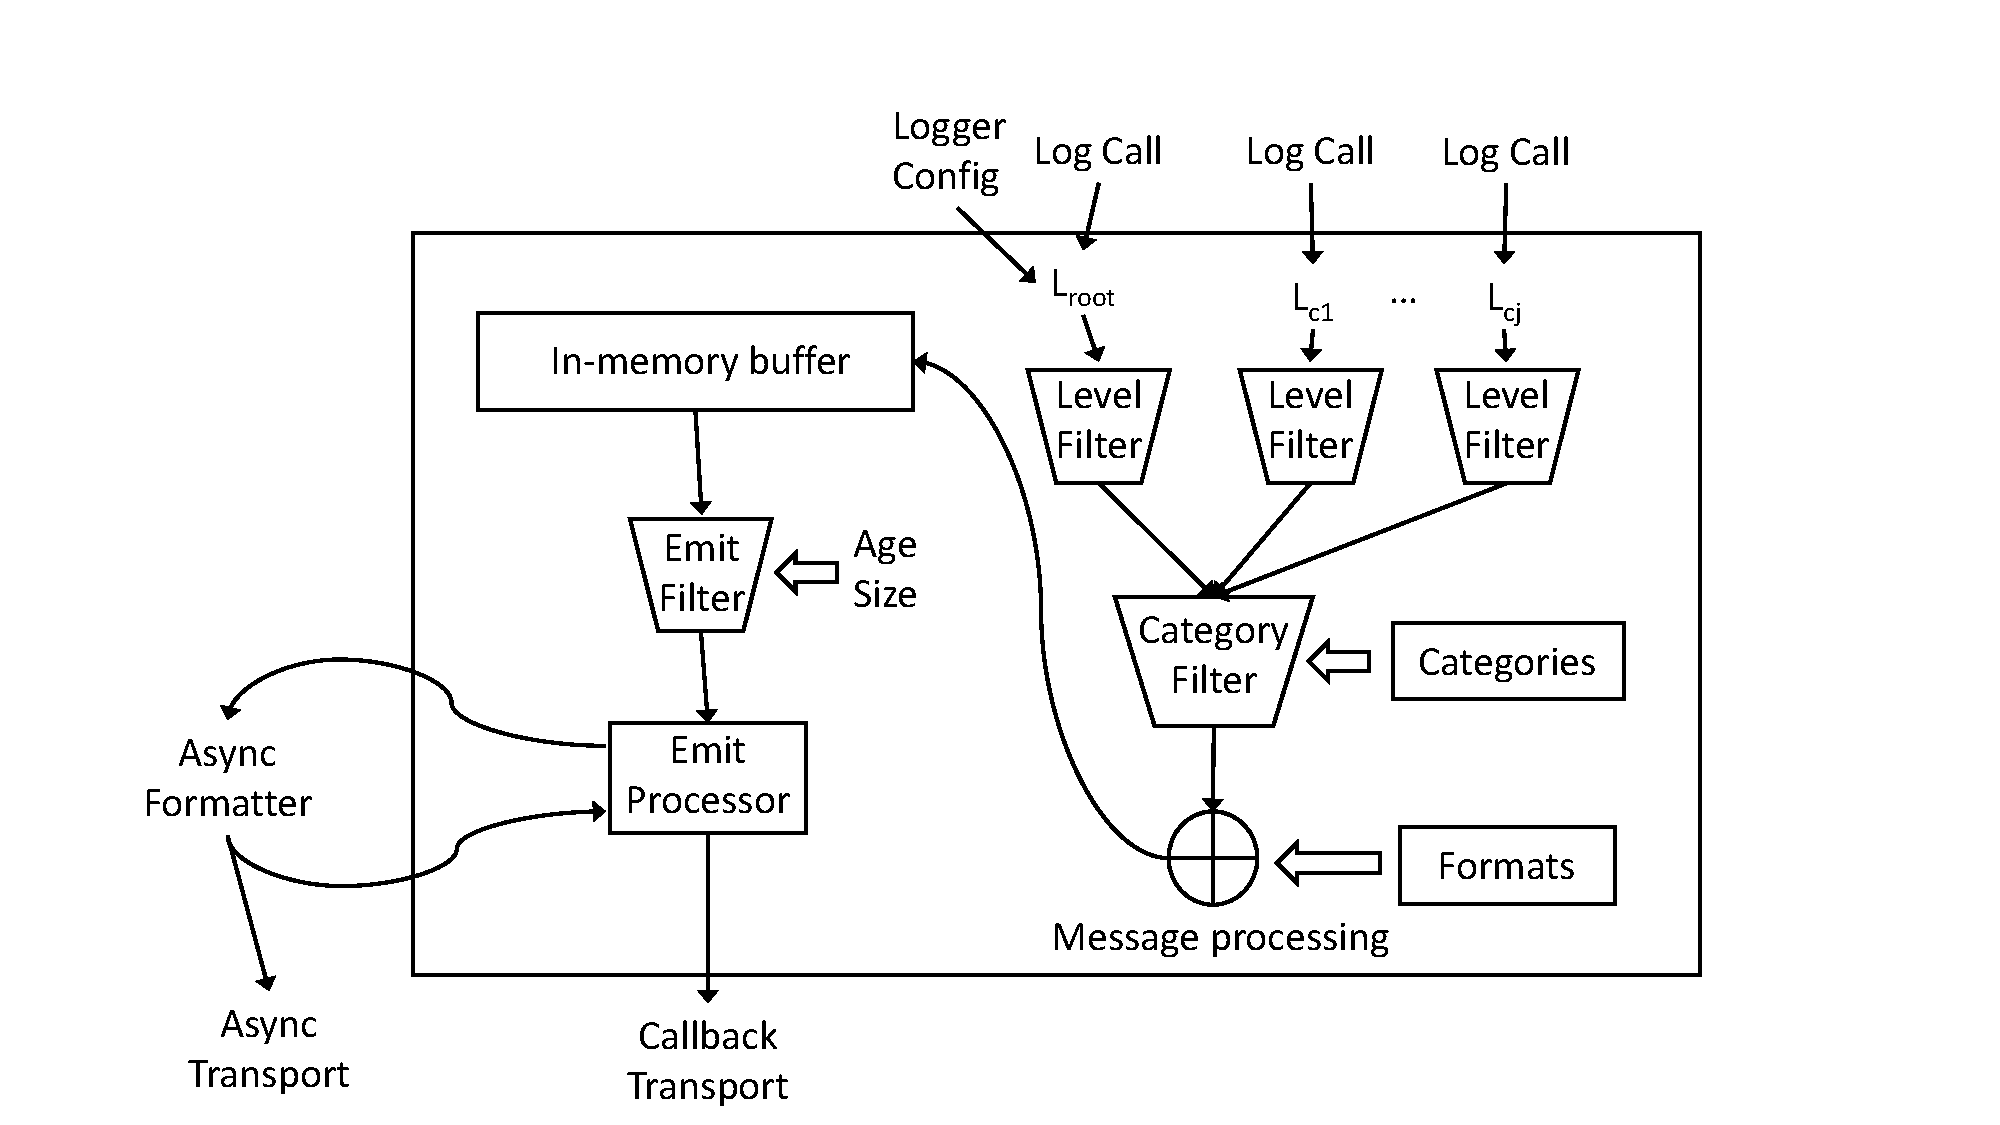
\includegraphics[width=0.5\textwidth,angle=-90]{Figures/ArchDiagram}
    \caption{Logger Architecture.}
    \label{fig:arch}
\end{figure}


\begin{figure*}[t]
\begin{minipage}[b]{0.5\textwidth}
    \lstinputlisting[language=JavaScript,basicstyle=\small]{runningExample.js} 
    \caption{Main app code.}
    \label{fig:appmain}
\end{minipage}
\begin{minipage}[b]{0.5\textwidth}
    \lstinputlisting[language=JavaScript,basicstyle=\small]{runningExampleSub.js}
    \caption{Submodule code.}
    \label{fig:appsub}
\end{minipage}
\caption{Running Example}
\label{fig:runningExample}
\end{figure*}

\subsection{JavaScript Implementation}
\paragraph{Log State Manager}
\noindent
The first component we look at in the implementation is the global log state 
manager. This component is responsible for tracking all of the loggers that 
have been created, which is the root logger, the enabled logging levels + 
categories, and the message formats which have been defined. 

As seen in~\autoref{fig:arch} and the running example may be many loggers 
created in different parts of the application. One logger is created on line 
2 of the main application~\autoref{fig:appmain} while a second is created 
in the module \texttt{foo.js} in~\autoref{fig:appsub} which is included from 
the main \texttt{app.js} file. ....


root/sub/child loggers

message formats

level/category checks and changes

\subsection{Native C++ Implementation}

Background N-API formatter

Background uploads

\subsection{Custom Runtime Implementation}

Format checking

Mutability checking

Code regen on level changes